\documentclass[a4paper,12pt,twoside]{article}
\usepackage[utf8]{inputenc}
\usepackage{graphicx}

\setlength{\paperwidth}{20,4cm}          
\setlength{\paperheight}{29,7cm}       
\setlength{\textwidth}{16cm}         
\setlength{\textheight}{24cm}        
\setlength{\topmargin}{-1.2cm}         
\setlength{\oddsidemargin}{0.40cm}   
\setlength{\evensidemargin}{0.40cm} 
\renewcommand{\baselinestretch}{1.4}

\begin{document}
	\begin{center}
		{\LARGE {Universidad Católica "Nuestra Señora de la Asunción" Campus Itapúa}}
	\end{center}
	\vspace*{0.1cm}
	\begin{center}
		{\large \rm \textbf {Facultad de Ciencias y Tecnologías}}
	\end{center}
	\vspace*{0.2cm}
	\begin{center}
		{\large \rm \textbf {Trabajo final de grado}}
	\end{center}		
	
	\baselineskip 30pt
	\vspace*{1cm}
	\begin{center}
		{\large \rm Entrenamiento de redes neuronales para la detección en tiempo real de amenazas y agresiones humanas en imágenes secuenciales}
	\end{center}

	\vspace*{1cm}

	\begin{center}
		{\sc  Gustavo Enrique Escobar Krug\\}
		\vspace*{0.1cm}
		
		\center{Docente tutor:}  
		\center{\sc Lic. Nidia Gagliardi}
	\end{center}
	
	\pagebreak
	
	\baselineskip 16pt

%%%%%%%%%%%%%%%%%%%%%%%%%%%%%%%%%%%%%%%%%%%%%%%%%%%%%%%%%%%%%%%%%%%%%%%%%%%%%%
	
\newpage
\setlength{\parskip}{1.3em}
\part{Estado del Arte}
\section{Introducción}
En la actualidad, la seguridad personal se está volviendo cada vez mas importante: los atracos, asaltos y robos se producen a plena luz del día, muchas veces a la vista de todos y de una manera cada vez mas violenta. La violencia utilizada durante estos actos es cada vez mayor, esto debido a múltiples factores tales como para evitar la resistencia de la víctíma, el tiempo en cometer el delito, etc. Las condiciones de seguridad existentes no parecen frenar esta violencia y hasta resulta inevitable en muchos casos. \par
Con el transcurrir de éstos últimos años, muchas personas y empresas dedicadas a la tecnología han centrado sus esfuerzos en ofrecer soluciones que puedan brindar ayuda incluso a los órganismos de seguridad. Las cámaras de circuito cerrado de televisión (CCTV) han tomado un protagonismo mas evidente en los sistemas de vigilancia dada la ventaja que ofrecen. \par

\subsection{Evolución de los sistemas de vigilancia}
A lo largo del tiempo, los sistemas de vigilancia ha mejorado la tecnología utilizada en los dispositivos de monitoreo, sensores, etc. Según M. Valera y S.A. Velastin. \cite{valera}, pueden diferenciarse hasta el momento tres generaciones de sistemas de vigilancia:
\begin{enumerate}
	\baselineskip 16pt
	\item Primera generación: \par 
	Consistían en cámaras de circuito cerrado analógicas que transmitían la señal de video en blanco y negro a través de un cable coaxial que se conectaba a un solo monitor. Entonces si tenías 10 cámaras, necesitabas 10 cables conectados a 10 monitores distintos. Un operador debía estar observando constantemente todos los monitores. \par 
	Con el transcurrir del tiempo, fueron introducidos los conmutadores, que eran dispositivos capaces de alternar la señal de video para transmitirla a un solo monitor \par  
	Esta tecnología, era incapaz de almacenar las imágenes, hasta la llegada de los VCRs (Video Camera Recorder) que grababan las imágenes en unidades de cinta (casettes). Los VCRs trajeron muchas ventajas a los sistemas de vigilancia pero aún así, la calidad de imágen almacenada era muy pobre, y con el tiempo tendía a estropearse. Con la llegada de la era digital, surgieron los dispositivos capaces de combinar y procesa múltiples señales de video almacenándolas en medios digitales: DVR (Digital Video Recorder). Los DVRs, que aún son utilizados en la actualidad, permiten la utilización de cámaras digitales para la captura de video, además de recibir varias señales de manera simultánea, también almacena las secuencias de video en formatos digitales, y además permite el acceso a través de redes IP.\\	
	
	\item Segunda generación: \par
	Con los sistemas de vigilancia computarizada, la utilización de diferentes sensores e inteligencia artificial deriva un concepto denominado Vigilancia Inteligente. Éste concepto, refiere a todos los componentes digitales que en su conjunto forman un sistema de vigilancia integral que responde a los estímulos captados por dichos componentes, prácticamente automáticos sin intervención humana. \par
	Ya no se trata de simples dispositivos analógicos o de cámaras antiguas conectadas a pantallas de rayos catódicos, sino que éstos sistemas utilizan dispositivos digitales y algoritmos computacionales para la extracción de datos a fin de detectar los estímulos que se producen en las señales transmitidas por los sensores o cámaras.
	\par
	La idea de éstos avances, es disminuir el trabajo realizado por agentes humanos, capaces de sufrir fatiga o cansancio, y sustituirlos por sistemas computacionales inteligentes que analicen en tiempo real los eventos captados por los distintos sensores y cámaras.\\
	
	\item Tercera generación: \par
	Los sistemas de vigilancia de tercera generació solo difieren de los de segunda en el modo en que se procesan los datos: es una red de proceso distribuido con múltiples cámaras/sensores. Esto ofrece robustez, ya que si una cámara/sensor deja de funcionar, el sistema sigue funcionando con los demás.
	\\
\end{enumerate}	\baselineskip 14pt



\subsection{Clasificación de los sistemas de vigilancia}

No todos los sistemas de vigilancia utilizan los mismos recursos y enfoques, la tecnología va mejorando los dispositivos con el transcurrir del tiempo, la integración de componentes digitales inteligentes acaparan los procesos de vigilancia. Y es importante conocer adecuadamente cada una de las clases de sistemas de vigilancia para entender la razón de éste trabajo.  \par

Dentro de la clasificación de sistemas de visión para vigilancia, R. Dautov et al \cite{dautov}. cita cuatro tipos distintos de sistemas de visión:
\begin{itemize}
	\item Sistemas de visión integrados: incluyen cámaras independientes, que realizan ASIP a bordo o en una unidad externa, como una computadora incorporada (ej., Raspberry Pi).\\	
	\item Los sistemas de visión basados en PC: cámaras inteligentes que consisten en una cámara de video y una computadora  realizando ASIP.\\	
	\item Los sistemas de visión basados en red: compuestas de múltiples cámaras interconectadas (ej., sistemas de vigilancia CCTV).\\	
	\item Los sistemas de visión híbrida: cámaras inteligentes, que pueden depender de la participación humana para proporcionar datos de alta precisión.\\	
\end{itemize}

\newpage
\part{Representación de poses}

\section{Postura y Pose humanas}

La postura es la forma natural que se establece con la disposición de las extremidades y el tronco del cuerpo humano. La pose, es la postura que sugiere la misma forma pero se dice que no es natural, es la postura de disposición artificial, buscada para cierto fin. \par

A través de la pose, el ser humano expresa una idea, una acción y hasta un mensaje reflejados en la forma dispuesta de todas las partes del cuerpo, y los ángulos formados entre sí. Se puede establecer entonces, a través de la pose, qué tipo actividad está realizando una persona humana con solo observarla en una imágen, por ejemplo. \par

\subsection{Elementos que conforman la pose}
Se utiliza el término pose, para referirse a la postura buscada de manera artificial para denotar una acción. Analizando el cuerpo humano y todos los movimientos realizables por el mismo, podemos citar los elementos mas importantes del cuerpo que son tomados en cuenta para establecer una pose: \begin{enumerate}
	\baselineskip 0pt
	\item Tronco del cuerpo (torso): pecho y caderas \\	
	\item Brazos y antebrazos: manos, codos y hombros \\
	\item Muslos y pantorrillas: pies, rodillas y caderas \\
\end{enumerate}	\baselineskip 14pt

\begin{figure}[h!]
	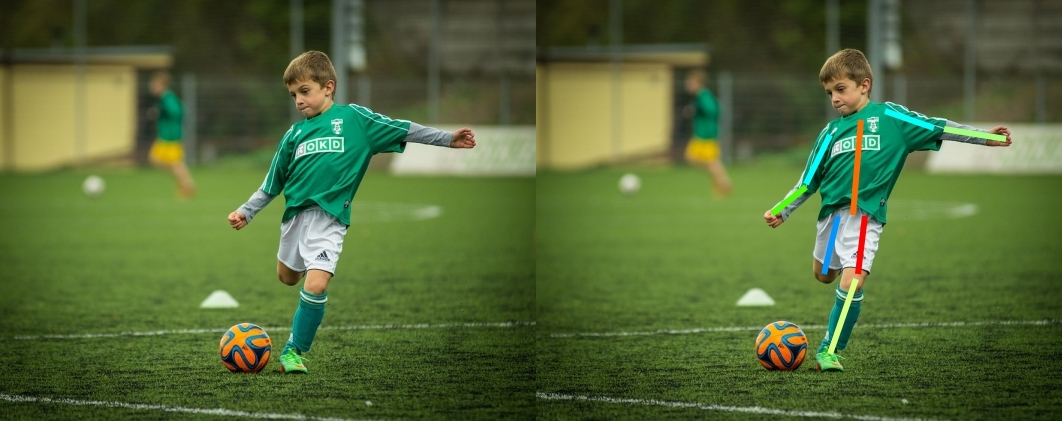
\includegraphics[width=\linewidth]{Imagenes/pose1.png}
	\caption{Pose humana. A la izq. la imagen original, a la der. se dibujan las líneas sobre los elementos mas importantes que conforman la pose. Fuente: pixabay.com}
	\label{fig:pose1}
\end{figure}

En la figura \ref{fig:pose1}, se muestra a un niño jugando al fúbtol. La pose establecida por el cuerpo del niño, sugiere una acción en concreto. Es posible determinar la acción ejecutada por el niño solemente observando la pose expresada en su cuerpo. \par

La configuración de la disposición de las extremidades, y su relación con el tronco del cuerpo humano, puede definir qué pose forma, y en la mayoría de los casos, la acción que se está ejecutando. \par

\subsection{Poses compatibles con amenazas y agresiones}
Si bien, determinadas poses pueden sugerir que el sujeto observado pueda estar realizando múltiples acciones, existen determinadas poses que son mayormente compatibles para acciones concretas: las amenazas y agresiones humanas.\par

Por amenazas y agresiones humanas, se entiende como la utilización de extremidades del cuerpo para proferir amenazas y agresiones físicas a cualquier objeto presente en su entorno, o la disposición de las extremidades de manera que el sujeto pueda estar utilizando un arma para efectuar una agresión o amenaza. \par 

Es posible que la agresión no sea efectuada hacia otra persona, o no se pueda visualizar qué o quién recibe la agresión, sin embargo se puede agredir a un objeto que pueda contener a un ser vivo dentro del mismo, ejemplo: una persona puede estar golpeando un auto, que en su interior contiene un niño (no visible para el observador).\par

Entonces, se pueden enumerar algunos ejemplos de poses que puedan ser considerada como una pose compatible con agresión humana:

\begin{enumerate}
	\baselineskip 0pt
	\item Brazos levantados formando ángulos de entre 50 y 120 grados con el tronco (ej. una persona apuntando un arma de fuego). \\	
	\item Brazos levantados formando ángulos superiores a los 170 grados con el tronco (ej. una persona propinando golpes con los brazos ) \\
	\item Muslos levantados formando ángulos cercanos a los 90 grados con el tronco (ej. una persona propinando golpes con sus piernas) \\
	\item Puede existir una combinación de lo anterior. \\
\end{enumerate}	\baselineskip 14pt

\begin{figure}[h!]
	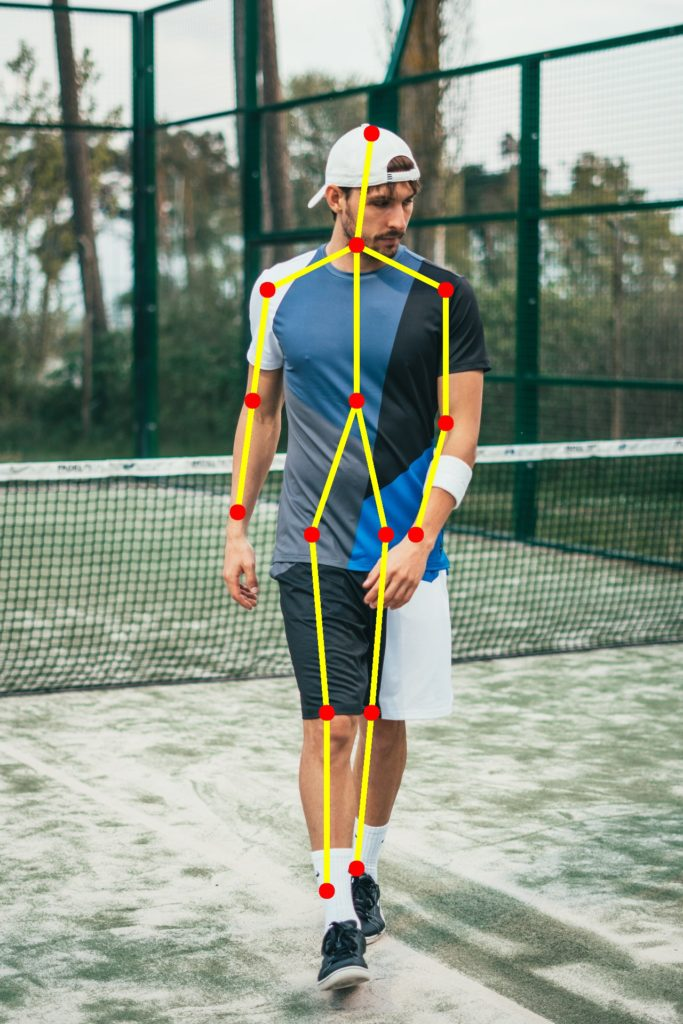
\includegraphics[width=220pt]{Imagenes/pose3.jpg}
	\caption{Pose humana compatible con agresión de brazos. Fuente: pixabay.com}
	\label{fig:pose3}
\end{figure}

En la \ref{fig:pose3} podemos observar a la persona del lado izquierdo con una amenaza mas compatible a una agresión que la persona del lado derechoo. Igualmente, ambas poses podrían ser compatibles con agresiones.\par

	
\newpage	
\part{Inteligencia Artificial}

\section{Conceptos de Machine Learning}

Se conoce como Machine Learning (en inglés), a la ciencia relacionada con Inteligencia Artificial en la cual se pueden configurar modelos matemáticos y probabilísticos para responder a situaciones de la vida real. Básicamente, se trata de entrenar algoritmos para ofrecer respuestas, esperadas o no, bajo ciertas condiciones de campo.\par
	
\subsection{Aprendizaje y entrenamiento}
El aprendizaje se da solamente en ciertos seres vivos del planeta, por lo que el concepto era ajeno a las máquinas, hasta ahora: consiste en incorporar conocimientos de situaciones repetitivas para poder responder con una acción o simplemente establecer un recuerdo del mismo.\par

En el ámbito de la computación, se adoptó el concepto de aprendizaje y entrenamiento al proceso de preparar y parametrizar, con datos de entrada, un modelo matemático o algoritmo para que pueda responder, con datos de salida, de la misma manera que lo haría un ser vivo capaz de aprender.\par

A partir de este punto, nos referiremos a los datos de entrada para el proceso de aprendizaje, como Input Dataset -o Dataset-, y la obtención de resultados de salida -o simplemente Output-.

\subsubsection{Aprendizaje supervisado}

Se conoce como aprendizaje supervisado al proceso de entrenar un algoritmo con datos de entrada estructurados, y en donde se conoce o se espera algún tipo de datos de salida previamente conocidos. En el aprendizaje supervisado, conocemos acerca de la naturaleza de los datos de entrada, y esperamos datos de salida del mismo modo. Por ejemplo, podemos estimar el costo de una casa a partir de ciertos datos conocidos, como el área, cantidad de pisos, ubicación, etc.\par

\subsubsection{Aprendizaje no supervisado}

Por el otro lado en el aprendizaje no supervisado, no conocemos la clasificación de los datos de entrada ni de salida. Los datos de entrada no poseen una estructura definida y no sabemos acerca de los datos de salida esperados. Datos de entrada para el aprendizaje no supervisado podrían ser: datos de audio, imágenes o texto. \par


\subsection{Clasificadores}

\subsubsection{Regresión Lineal}

La regresión lineal es un tipo de clasificador binario, solo devuelve dos posibles datos de salida: 1 o 0. Este tipo de clasificador se utiliza para determinar si un objeto es o no es de cierto tipo.

Si se dibujaran los datos en un gráfico de absisas, podríamos separar los valores para 1 y 0 por medio de una línea -denominada límite de decisión-.

Una unidad de datos de entrenamiento puede identificarse como (x, y) donde x representa los datos de entrada, e y representa el de salida esperado. 

\begin{figure}[h!]
	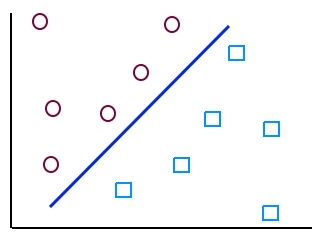
\includegraphics[width=220pt]{Imagenes/regresion1.jpg}
	\caption{Regresión lineal, datos de salida en un gráfico de absisas con el límite de desición}
	\label{fig:regresion1}
\end{figure}


\subsubsection{Regresión Logística}

La regresión logística también es un clasificador binario, pero se diferencia de la Regresión Lineal en que los datos, en el gráfico de absisas, están separados por una línea cuadrática. \par

\begin{figure}[h!]
	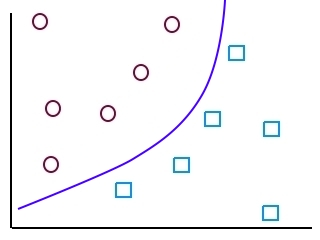
\includegraphics[width=220pt]{Imagenes/regresion2.jpg}
	\caption{Regresión logística, datos de salida en un gráfico de absisas con el límite de desición}
	\label{fig:regresion2}
\end{figure}


\subsubsection{Redes Neuronales}

En biología, una neurona es una célula del sistema nervioso que es capaz de comunicar pulsos eléctricos a otras células. \par


A DESARROLLAR


\newpage
\part{Procesamiento gráfico}

\section{Visión por computadora}
En los últimos años, los problemas de visión por computadora han acaparado la mayoría de los trabajos e investigaciones dada la cantidad de situaciones en las cuales es necesario utilizar ayuda no humana para resolverlas. Los sistemas computacionales han evolucionado y la inteligencia artificial ha surgido como una ciencia de estudio capaz de proveer la ayuda necesaria. \par

Sin embargo, un conjunto de componentes electrónicos no es capaz de entender una imágen. La representación de una imagen, en términos informáticos, es la agrupación de números distribuidos en una matriz.\par

En esta sección, se expondrán los principios básicos, componentes y operaciones fundamentales que surgen alrededor del procesamiento de imágenes por computadora.\par


\subsection{Detección y reconocimiento de objetos en imágenes}

Los sistemas de vigilancia en auge actualmente son los de segunda generación: dispositivos que capturan imágenes que son enviadas a procesadores que utilizan algoritmos computacionales para obtener la información relevante de las mismas. \par

Si bien existen investigaciones enfocadas a la utilización de Inteligencia Artificial para la Vigilancia Inteligente, ésto resulta por ahora una tarea difícil de implementar debido a la cantidad de combinaciones posibles de escenarios que puedan darse, la cantidad de datos de entrada y los patrones que se deben analizar en las diferentes fases. Normalmente, el proceso de identificación de objetos en imágenes se da en diferentes etapas descritas en \cite{lozano} y \cite{kamarudin}, ellas son:	
\begin{enumerate}
	\baselineskip 0pt
	\item Detección de objetos.\\	
	\item Clasificación (identificación) de objetos.\\
	\item Extracción de características de objetos (features).\\
	\item Análisis del comportamiento de los objetos.\\
\end{enumerate}	\baselineskip 14pt


\subsubsection{Detección de objetos en imágenes}
La detección de objetos en imágenes es una de las áreas de mayor investigación en visión por computadora. La tarea no resulta fácil, ya que existen numerosos elementos a tener en cuenta para la detección de objetos que sean de relevancia. \par
El principal obstáculo, es determinar si un conjunto de pixeles forman o no un objeto tomando en cuenta que existen innumerables combinaciones de posición, luminosidad, color y formas, como asi tambien el ruido de interferencia y el tamaño del objeto (o su lejanía de la cámara).\par
Enfocado a la seguridad, la detección de objetos trata de identificar solamente unas pocas categorías de objetos en imágenes, lo que lo hace un proceso mas viable: la detección de formas humanas, también denominado detección de peatones (Pedestrian detection \cite{zhang1}).

\subsubsection{Técnicas de detección de objetos en imágenes}
A través de los años, como consecuencia de las investigaciones en visión por computadora, han surgido	diferentes enfoques en la utilización de técnicas de detección de objetos, M. Valera y S.A. Velastin \cite{valera} citan dos enfoques a lo que se pueden agregar ademas el presentado en \cite{nidhi} y el citado en \cite{barron}:
\begin{enumerate}
	\baselineskip 0pt
	\item Diferencia temporal: 
	este enfoque se basa en la comparación de un frame (imágen de video) con el frame anterior. Esta acción permite identificar objetos en movimiento cambiante dentro del conjunto de frames, aunque sugieren que es un proceso mas lento que otros.\\	
	\item Substracción de fondo: utiliza una imagen de fondo que se compara con frames pixel a pixel para determinar los cambios ocurridos en la imagen, lo que permite obtener contornos de objetos.\\
	\item Filtrado: este método es quizás el menos utilizado ya que las características de los objetos suelen ser variantes. Este método sugiere la detección de objetos basados en el filtrado de color del mismo: se extraen los pixeles que concuerdan con el color de un objeto previamente establecido. Como los objetos pueden variar su color, o luminosidad, este método resulta poco efectivo. Puede utilizarse en condiciones muy controladas.\\
	\item Flujo óptico: este método es el más costoso computacionalmente hablando, ya que determina vectores de movimiento de cada uno de los pixeles para determinar el contorno de un objeto en movimiento dentro de un frame. Cada pixel en movimiento (posición inicial y posición final) determina un vector, un sentido de movimiento. Se puede tomar el conjunto de vectores de todos los pixeles para determinar la existencia de un objeto en la imágen.\\
\end{enumerate}	\baselineskip 14pt

\subsubsection{Clasificación de objetos}
La última etapa, luego de la detección de objetos, es la clasificación de los mismos: se debe determinar la clase de objeto detectado. Es de vital importancia poder indentificar el tipo de objeto detectado, especialmente cuando se trata de personas: necesitamos registrar y catalogar el comportamiento de objetos de tipo persona para determinar si se produce una forma compatible de agresión.
\subsubsection{Técnicas de clasificación}
Para determinar la clase de objeto extraído de una imágen, se utilizan dos tipos principales de técnicas citadas por \cite{lozano}:
\begin{enumerate}
	\baselineskip 0pt
	\item Clasificación basada en formas: es la técnica mas sencilla y consiste en, una vez identificado un objeto en una imágen, compararlo con formas de objetos existentes. Se asocia un valor numérico para identificar el grado de similitud entre las imágenes comparadas. El valor más alto asociado definirá la clase de objeto.\\
	\item Clasificación basada en movimiento: estudia el movimiento hecho por un objeto en particular, con respecto a su forma o silueta. Se sabe por ejemplo, que el cuerpo humano va cambiando su forma -esto es, existe movimiento- a través de las imágenes. Todo lo contrario a lo que ocurre con los automóviles, que no suelen cambiar su forma.
	\\
\end{enumerate}	\baselineskip 14pt

\subsubsection{Métodos de clasificación}
Ya hemos citado las técnicas que mayormente se utilizan en la clasificación de objetos, además de que existen otras técnicas menos conocidas o que producen resultados menos certeros, ahora hay que hablar sobre los métodos de clasificación utilizados actualmente por programas computacionales para separar objetos según su clase utilizando las técnicas citadas previamente.
S. Bailey et al \cite{bailey} describe algunos métodos principales de clasificadores, también podemos agregar los citados por N. S. Kamarudin et al\cite{kamarudin}, y aunque no ahondaremos en ellos, necesariamente debemos citarlos a fin de poder comprender la metodología de clasificación utilizada en este trabajo. A continuación, algunos de los métodos de clasificación más conocidos son:
\begin{enumerate}
	\baselineskip 0pt
	\item Medidas de probabilidad multidimensionales: este modelo utiliza la Función De Probabilidad de Distribución para determinar, mediante funciones matemáticas de probabilidad, la distribución de ciertas características de un objeto en una imágen y asi poder establecer la clase de objeto. La probabilidad combinada de todos los valores de las características de un objeto es utilizada para establecer ciertos parámetros de decisión.\\
	\item Árboles de decisiones, en inglés 'Decision Trees': modelo utilizado para separar ciertos criterios o características de objetos y eventos ocurridos en el fondo de la imágen. Éste modelo permite hacer un corte mas preciso sobre qué características se obtienen del objeto de estudio y asi poder determinar su clasificación.\\
	\item Máquinas de vectores de soporte, en inglés 'Support Vector Machines' (SVM): es un método de clasificación que utiliza funciones matemáticas gráficas: dado un conjunto de puntos donde cada uno pertenece a una de dos posibles categorías, se construye un modelo capaz de predecir si un punto nuevo pertenece a de las dos categorías. Básicamente, una linea recta o curva, separa los puntos de entrenamiento en dos áreas diferentes en un gráfico. Mediante una función matemática, podemos determinar si un dato de entrada (nuevo punto) pertenece o no a uno de los dos grupos establecidos mediante la separación realizada.\\
	\item Redes bayesianas: es un modelo de grafo probabilístico que representa un conjunto de variables y sus relaciones condicionales. Básicamente, funciona de la misma manera que un árbol de decisiones, pero en las redes bayesianas, la estructura gráfica cambia y no existen niveles de nodos: las caraterísticas pueden estar conectadas unas con otras formando un grafo dirigido. A medida que se van cumpliendo ciertas variables para un objeto, puede determinarse -siguiendo el grafo- a que clase de objeto pertenece.\\
	\item Redes Neuronales Artificiales: la utilización de redes neuronales para clasificación es uno de los métodos mas utilizados actualmente. Éstas simulan la interconexión de las neuronas cerebrales. Las redes neuronales asignan un conjunto de variables de entrada a diferentes resultados de salida a través de nodos intermedios por los cuales van circulando los datos. Los nodos intermedios pueden ser muchos, o simplemente pueden no existir, dependiendo de las necesidades del modelo.\\
\end{enumerate}	\baselineskip 14pt	
	
\section{Herramientas de visión por computadora}

\subsection{OpenCV}

OpenCV (Open Computer Vision, en inglés) es una librería escrita con participación de investigadores de Intel Corp. para el procesamiento de imágenes por computadora según lo descrito en la referencia oficial \cite{opencv1}. Provee una serie de procedimientos y funciones estándar para la manipulación de imágenes en, hasta ahora, tres lenguajes de programación de computadoras: C++,  Python y Java. Provee herramientas preestablecidas y preconfiguradas para que la tarea del programador sea mas fácil y eficiente. \par

OpenCV se escribió con la finalidad de ser eficiente y aprovechar las instrucciones de bajo nivel de los procesadores Intel, que son los más vendidos en el mercado. Esto, sumado a que fue escrito en C++, hace que el código se ejecute mucho mas rápido que otras librerias de procesamiento de imágenes.\par

Además, la librería ofrece bibliotecas de funciones y procedimientos parametrizables para resolver problemas de Inteligencia Artificial. Los componentes prefabricados con un alto nivel de abstracción hacen posible al programador implementar, por ejemplo, un clasificador de objetos en unas pocas líneas de instrucciones Python.\par

Módulos de Inteligencia Artificial disponibles en OpenCV:
\begin{itemize}
	\item Clasificadores en cascada\\	
	\item Clasificadores Bayes\\	
	\item Support Vector Machines\\	
	\item Decision Trees \\	
	\item Redes neuronales \\	
\end{itemize}

En este trabajo, no se explicarán ni detallarán sobre los módulos de tratamiento de imágenes de OpenCV, ya que no se utilizaron durante el desarrollo. En su lugar, se abordarán conceptos y detalles sobre algunos de las librerías OpenCV de Inteligencia Artificial que fueron utilizados.\par

\subsubsection{Clasificadores en Cascada}

Llamados en inglés 'cascade of boosted classifiers working with haar-like features', es un módulo OpenCV que implementa una serie de clasificadores que generalmente son utilizados para detección de objetos en imágenes. Una serie de clasificadores simples están dispuestos en una estructura de cascada de manera que puedan funcionar más rapidamente que un clasificador único y pesado.  \par

La palabra boosted además, hace referencia a que estos clasificadores implementan técnicas que aceleran la ejecución de manera eficiente, actualmente se implementan cuatro técnicas conocidas como: Discrete Adaboost, Real Adaboost, Gentle Adaboost y Logitboost. No se detallarán sobre estas técnicas en el presente documento.\par

Las entradas de datos para los clasificadores, se conocen en inglés como 'Haar-like features'. Cada clasificador simple que compone la cascada recibe solo un tipo de entrada (feature), que en combinación con los demas clasificadores, pueden determinar la clase de objeto en proceso. La entrada es un conjunto de pixeles con una distribución en particular, como se detalla en la siguiente imagen.\par

\begin{figure}[h!]
	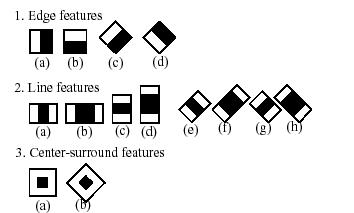
\includegraphics[width=300pt]{Imagenes/haarlike.jpg}
	\caption{Entradas (Features) para los distintos clasificadores en cascada Fuente: OpenCV Reference Manual}
	\label{fig:haarlike1}
\end{figure}

\subsubsection{Redes Neuronales Artificiales Convolucionales}

A desarrollar
















	
\newpage	
\begin{thebibliography}{9}
	\bibitem{valera} 
	M. Valera, S.A. Velastin. \textit{Intelligent distributed surveillance system: a review. IEE Proc. Vis. Image Signal Process.} 152(3):192–204, 2005.
	
	\bibitem{dautov} 
	1.R. Dautov, S. Distefano, D. Bruneo, F. Longo, G. Merlino, A. Puliafito, R. Buyya. \textit{Metropolitan intelligent surveillance systems for urban areas by harnessing IoT and edge computing paradigms.} 48(2):1475–1492, 2018.

	\bibitem{lozano} 
	M. D. Ruiz Lozano. \textit{Un modelo para el desarrollo de sistemas de detección de situaciones de riesgo capaces de integrar información de fuentes heterogéneas. Aplicaciones.} Granada, 2010.

	\bibitem{zhang1} 
	Zhang, G.D., Jiang, P.L., Matsumoto, K., Yoshida, M. and Kita, K. \textit{An Improvement of Pedestrian Detection Method with Multiple Resolutions.} Journal of Computer and Communications. 5(1) 102-116, 2017

	\bibitem{nidhi} 
	Nidhi. Dept. of Computer Applications, NIT Kurukshetra, Haryana, India. \textit{Image Processing and Object Detection.} International Journal of Applied Research 2015; 1(9): 396-399, 2015.
	
	\bibitem{barron} 
	J.L. Barron, D.J. Fleet, S.S. Beauchemin \textit{Performance of Optical Flow Techniques.} IJCV 12:1 pp43-77, 2015.
	
	\bibitem{kamarudin} 
	N. S. Kamarudin, M. Makhtar, S. A. Fadzli, M. Mohamad, F. S. Mohamad, M. F. A. 
	Kadir \textit{Comparison of Image Classification Techniques using Caltech 101 Dataset.} Journal of Theoretical and Applied Information Technology, 71(2):1992-8645, 2015.
	
	\bibitem{bailey} 
	S. Bailey, C. Aragon, R. Romano, R. C. Thomas, B. A. Weaver, D. Wong \textit{How to find more Supernovae with less work: Object Classification Techniques for Difference Imaging.} Journal of Theoretical and Applied Information Technology, 665(2):1246-1253, 2007.	
	
	\bibitem{opencv1} 
	Intel Corp. \textit{The OpenCV Reference Manual, Release 3.0.0-dev} 2014.	
	
	
	
\end{thebibliography}

\end{document}